%%利用XeLaTeX编译两次生成目录
\documentclass{ctexart}%%中文文档类型
\usepackage{amsmath,amsthm}%%美国数学会宏包
\newtheorem{exer}{{定理}}%[section]%定义一个练习环境
\usepackage{graphicx}%%插图宏包
\usepackage[super,square]{natbib}%%参考文献引用格式调整
\usepackage{listings}
\usepackage{algorithm}
\usepackage{float}%%固定图片位置,使用参数H

%%并排放两张图片的包
\usepackage{subfig}%多个子图
\usepackage{caption}%注释设置



\usepackage{algpseudocode}
\lstset{language=Matlab}%代码语言使用的是matlab
\lstset{breaklines}%自动将长的代码行换行排版
\lstset{extendedchars=false}%解决代码跨页时,章节标题,页眉等汉字不显示的问题


%colorlinks就是说超链接是否带颜色;
%linkcolor就是目录,公式,图表等内部链接的颜色;
%filecolor就是文件型链接的颜色;
%urlcolor就是网页链接的颜色;
%citecolor就是参考文献连接的颜色;
\usepackage{hyperref}
\hypersetup{hidelinks,
	colorlinks=true,
	allcolors=black,
	pdfstartview=Fit,
	breaklinks=true,
	linkcolor=cyan,
	filecolor=blue,      
	urlcolor=red,
	citecolor=green}

% Windows系统使用
%\usepackage{xeCJK}
%\setCJKmainfont{SimSun}

% Mac系统使用
\usepackage{xeCJK}
\setCJKmainfont[BoldFont=STHeiti,ItalicFont=STKaiti]{STSong}
\setCJKsansfont[BoldFont=STHeiti]{STXihei}
\setCJKmonofont{STFangsong}


\title{\LaTeX 排版艺术}%%论文标题
\author{quxk}

%自定义时间
%\date[06/13/17]{2017年6月13日} 

%系统时间
\date{\small \today \ \\ {\it}}

%隐藏时间
%\date{}

%%以上都是导言区
\begin{document}
\maketitle %%生成标题等信息

\begin{abstract}%% 摘要
	好好学习,天天向上。	
	\textbf{关键词:} study, up
\end{abstract}

\newpage %%另起一页
\tableofcontents%%生成目录




%% 插入数学公式
\newpage
\section{数学公式}
%% 数学公式等
数学公式$c^2=a^2+b^2$,以及
$$\sum_{n=1}^\infty \frac1{n^2}=\frac{\pi^2}6.$$
或者
\[\sum_{n=1}^\infty \frac1{n^2}=\frac{\pi^2}6.\]

没编号的公式
\begin{align*}
\sqrt{a^2 + b^2} &= c^2,\\
\sum_{n=1}^\infty \frac1{n^2}&=\frac{\pi^2}6.
\end{align*}

有编号的公式
\begin{align}\label{eq:1}
\sqrt{a^2 + b^2} &= c^2,\\
\sum_{n=1}^\infty \frac1{n^2}&=\frac{\pi^2}6.\label{eq:2}
\end{align}
其中\eqref{eq:1}和 \ref{eq:2} 都是很熟知的公式.

错误输入
\[
\{\sin(\frac{\pi}{6}+1)+1\}\ln 2.
\]

正确输入
\[
\left\{\sin\left(\frac{\pi}{6}+1\right)+1\right\}\ln 2.
\]

%% 插入图片
\newpage
\section{插入图片}

%%单张图片插入
\begin{figure}[!htb]
	%其中!h只是试图将图片放在当前位置,如果页面剩下的部分放不下,还是会跑到下一页的(t)顶部或者(b)底部。
	%H借助float包可以固定图片位置
	\centering
	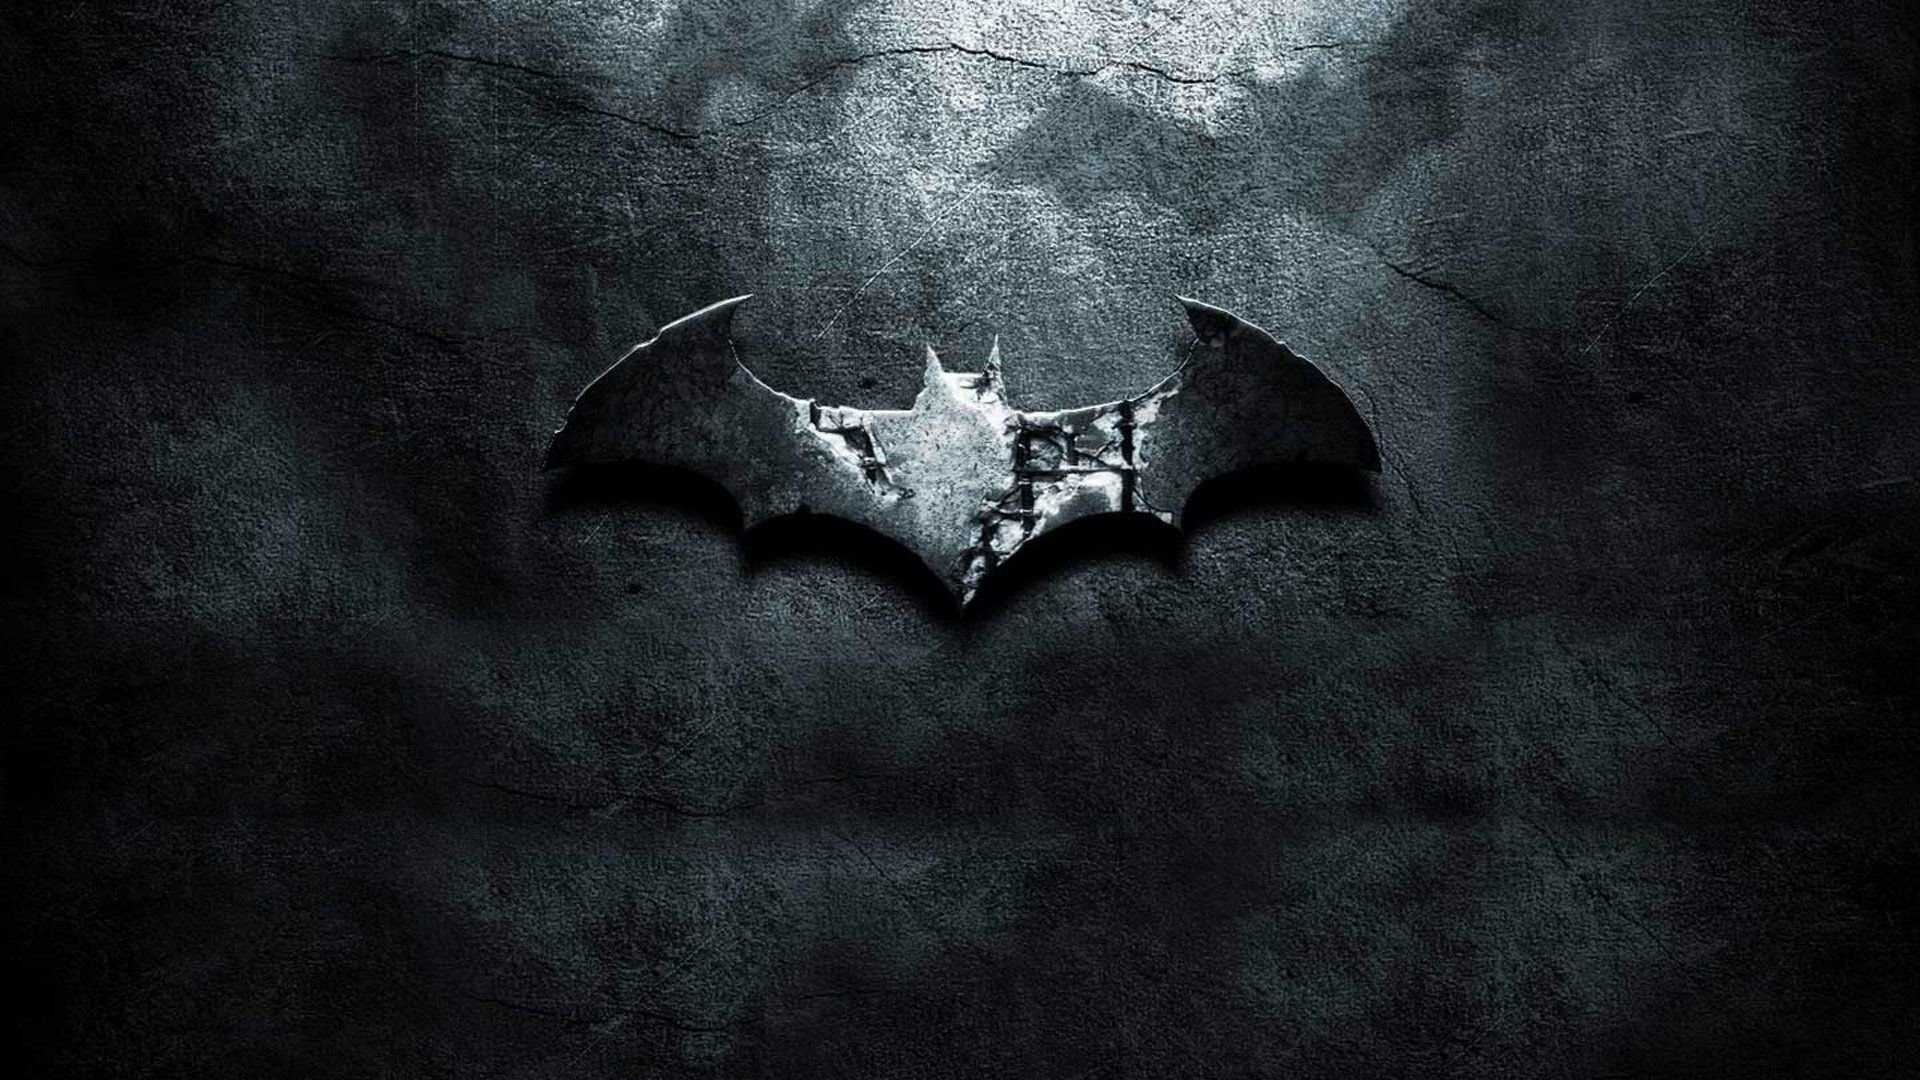
\includegraphics[width = 0.7\linewidth]{./pictures/94.jpg}
	\caption{蝙蝠侠}\label{fig:1}
\end{figure}

%%并排两张图片插入

\begin{figure}[htbp]  %[htbp]中的h是浮动的意思
	\centering    %居中
	\subfloat[蝙蝠侠] %第一张子图
	{
		\begin{minipage}[t]{0.5\textwidth}
			\centering%子图居中
			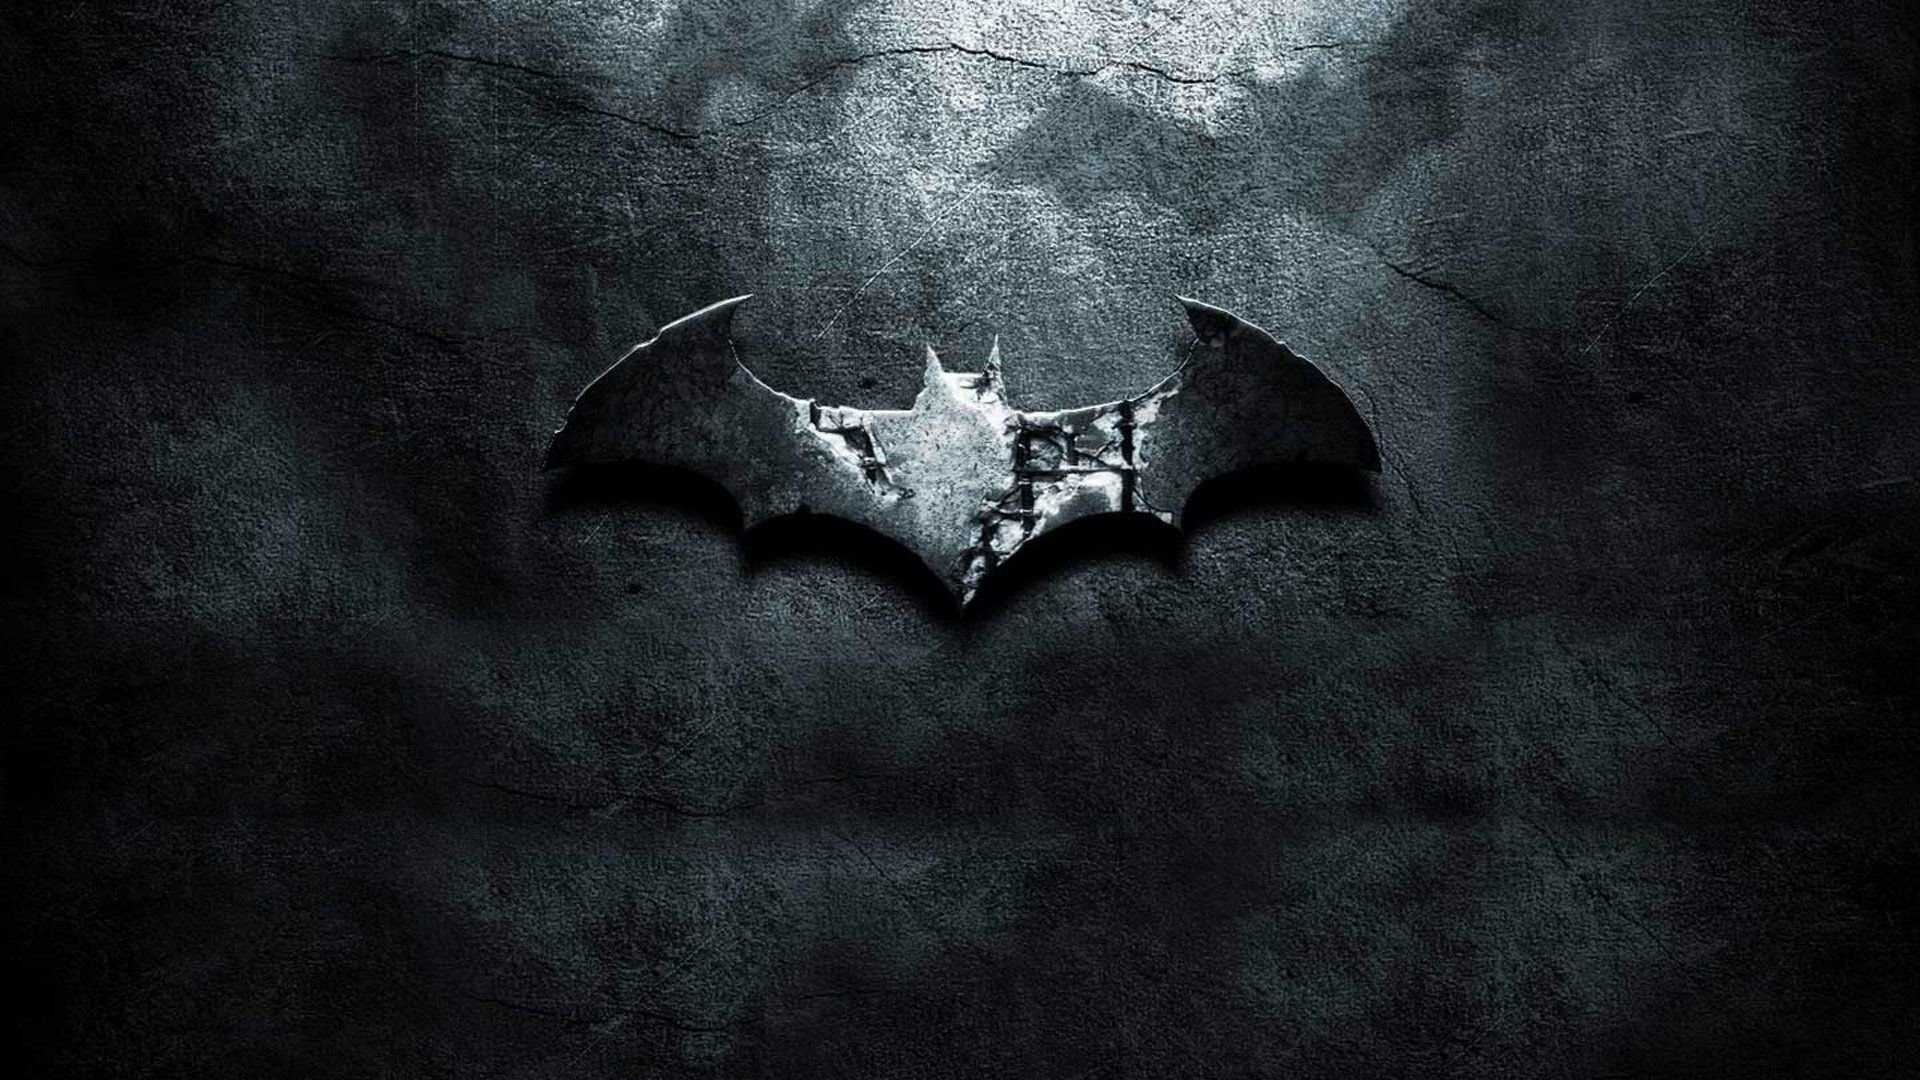
\includegraphics[width=0.65\textwidth]{./pictures/94.jpg}   %以行宽的0.5倍大小显示
			\label{fig1}
		\end{minipage}%
	}%注意这里不能回车空行,否则两张图会上下排列,而不是并排排列
	\subfloat[钢铁侠] %第二张子图
	{
		\begin{minipage}[t]{0.5\textwidth}
			\centering      %子图居中
			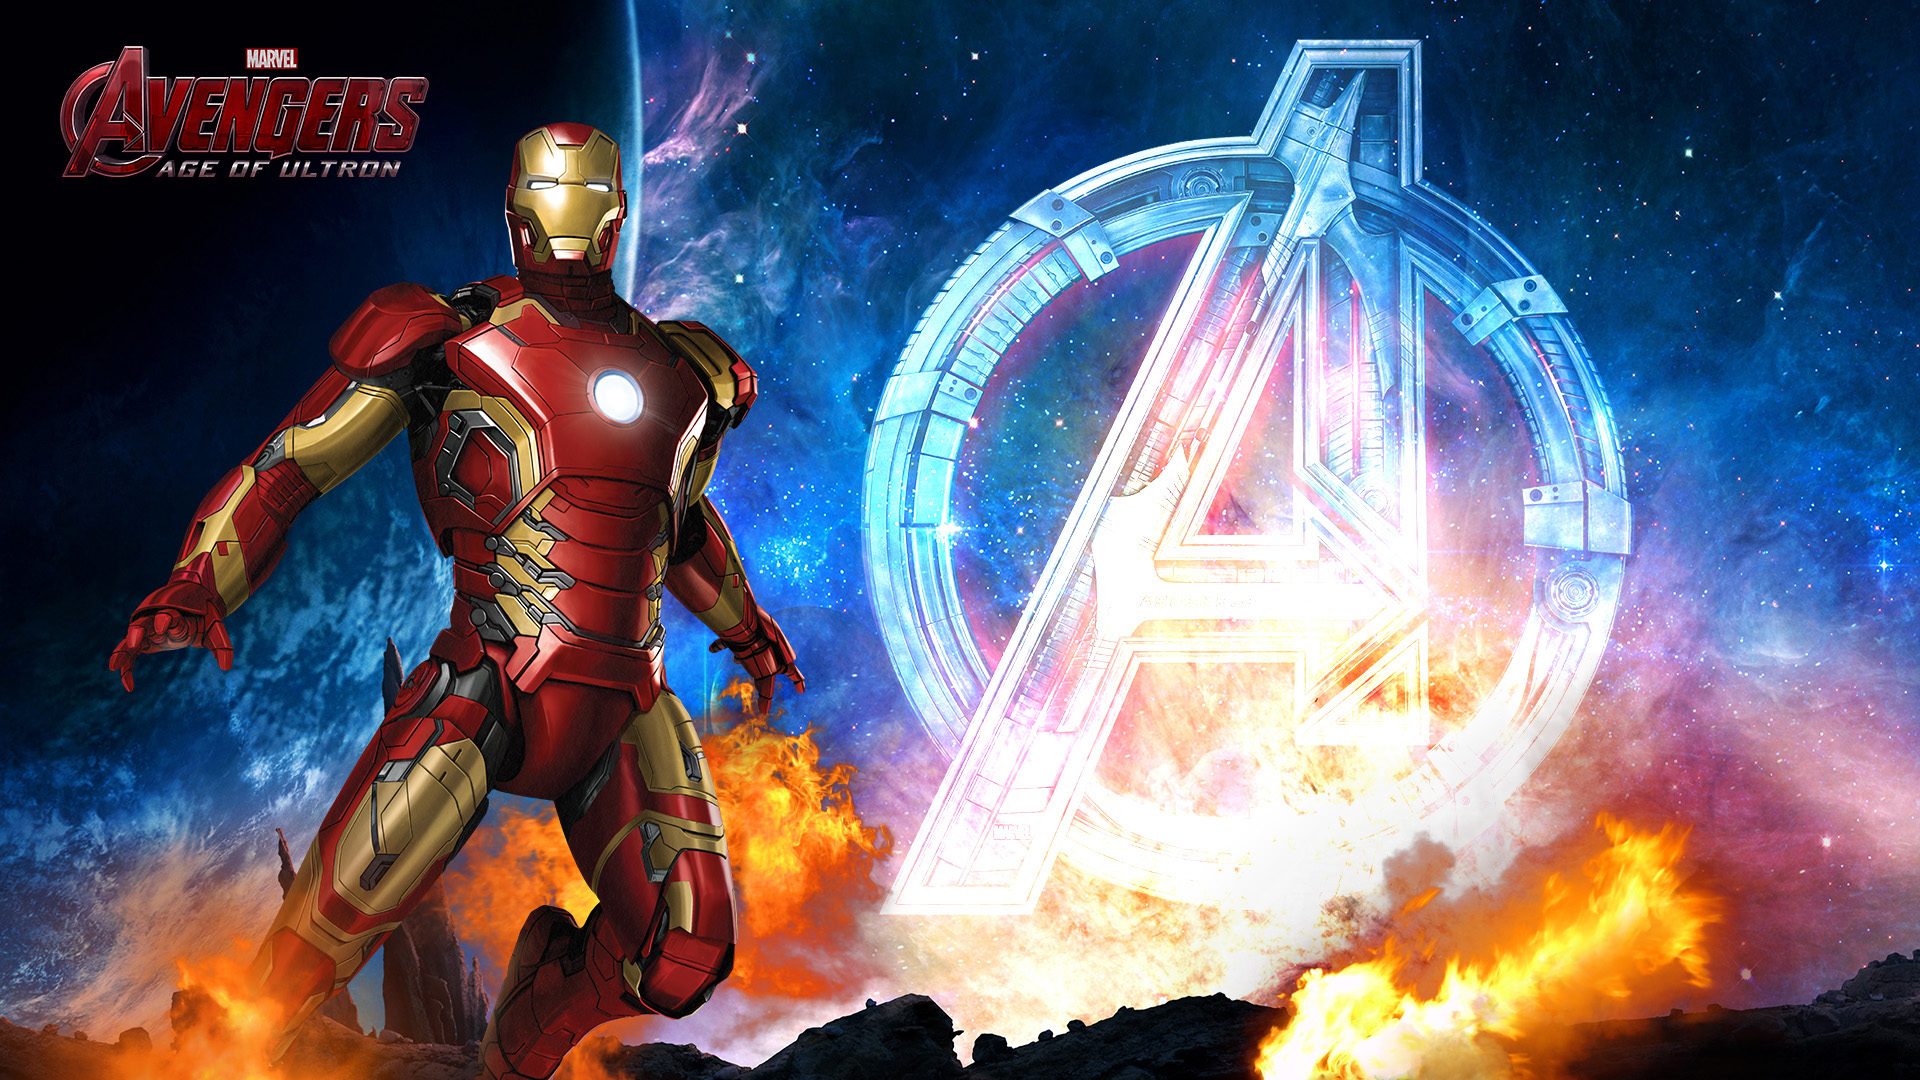
\includegraphics[width=0.65\textwidth]{./pictures/6.jpg}   %以行宽的0.5倍大小显示
			\label{fig2}
		\end{minipage}
	}
	\caption{Schematic diagram of a four-level tripod-type atomic system driven by three coherent laser fields.} %  %大图名称
	\label{FIG}  %图片引用标记
\end{figure}
图片 \ref{fig1} 是蝙蝠侠,图片 \ref{fig2} 是钢铁侠,图片 \ref{FIG} (a)是蝙蝠侠。



%% 插入2*2排列图片,m*n类似,用 \quad 来换行
\begin{figure}[htbp]
	\centering
	\subfloat[SubCaption\_1]
	{
		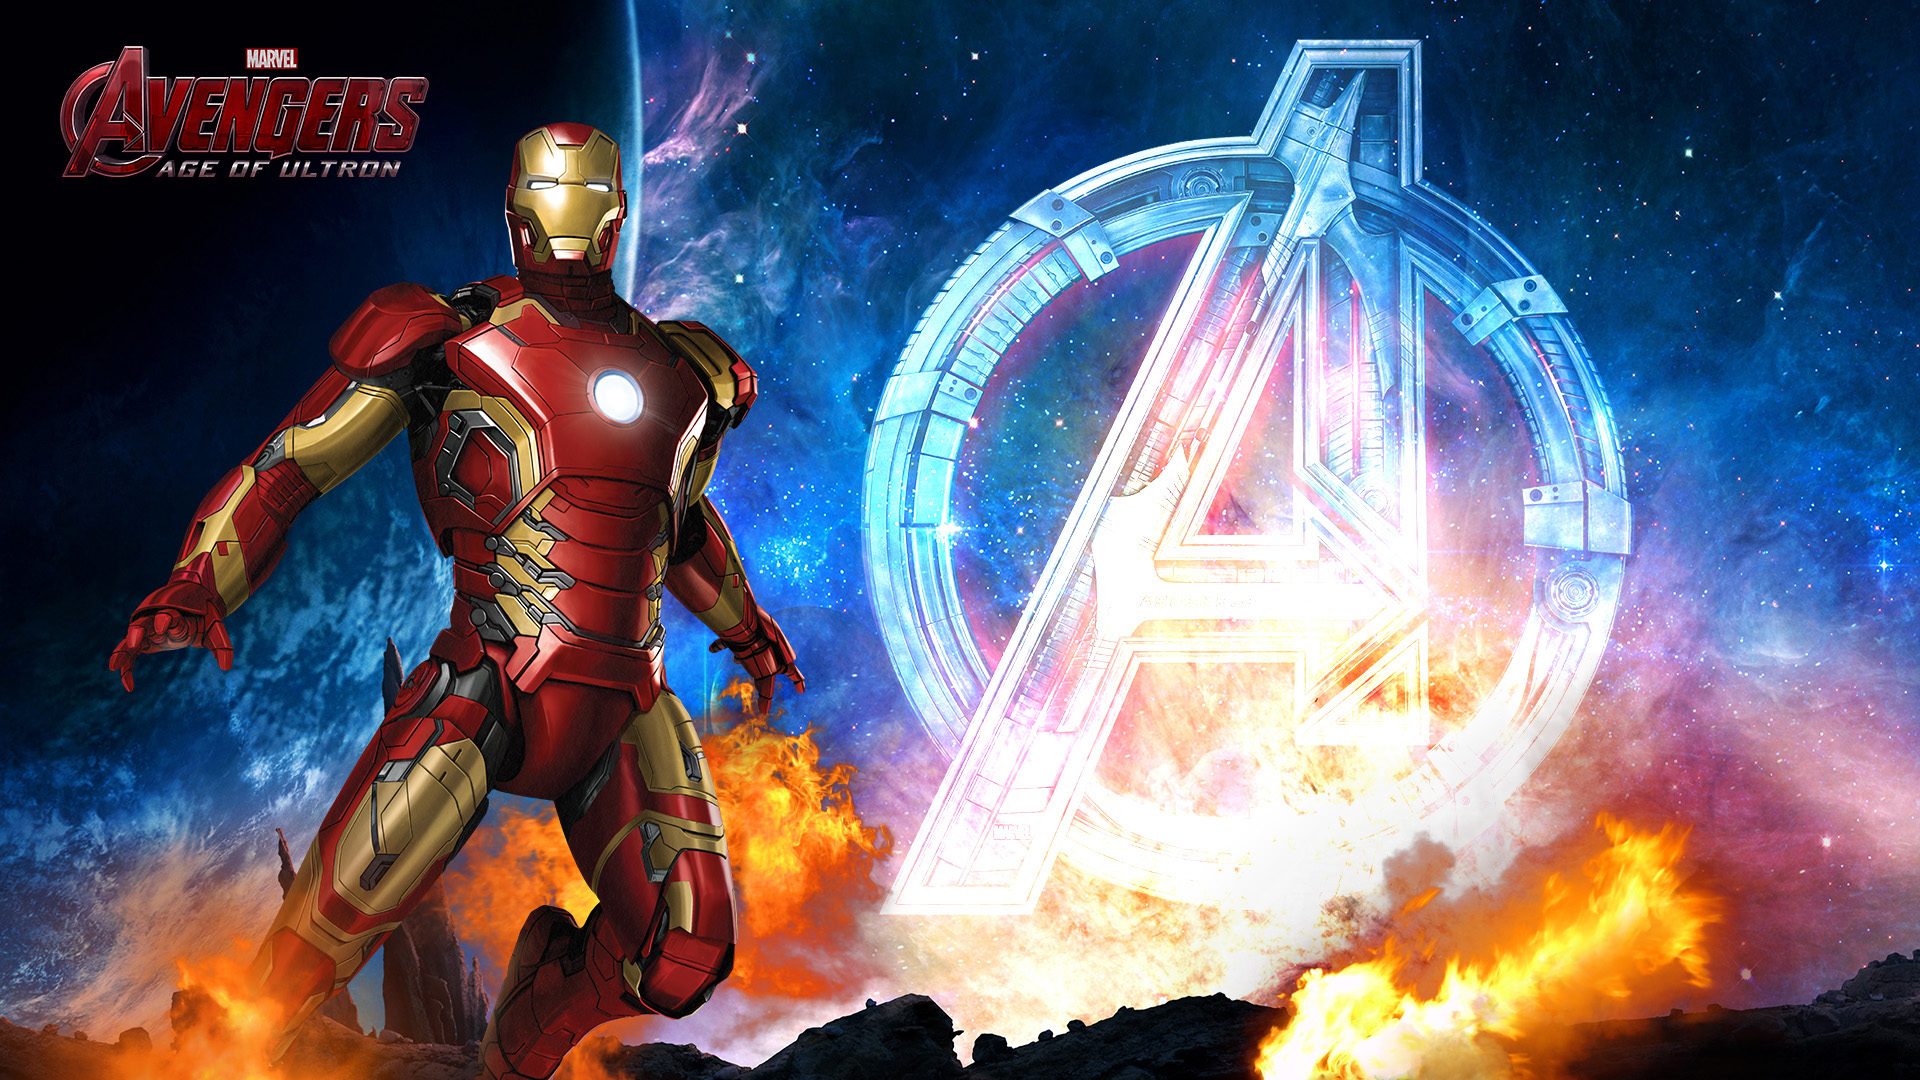
\includegraphics[width=2.5in]{./pictures/6.jpg}
		\label{label_for_cross_ref_1}
	}
	\subfloat[SubCaption\_2]
	{
		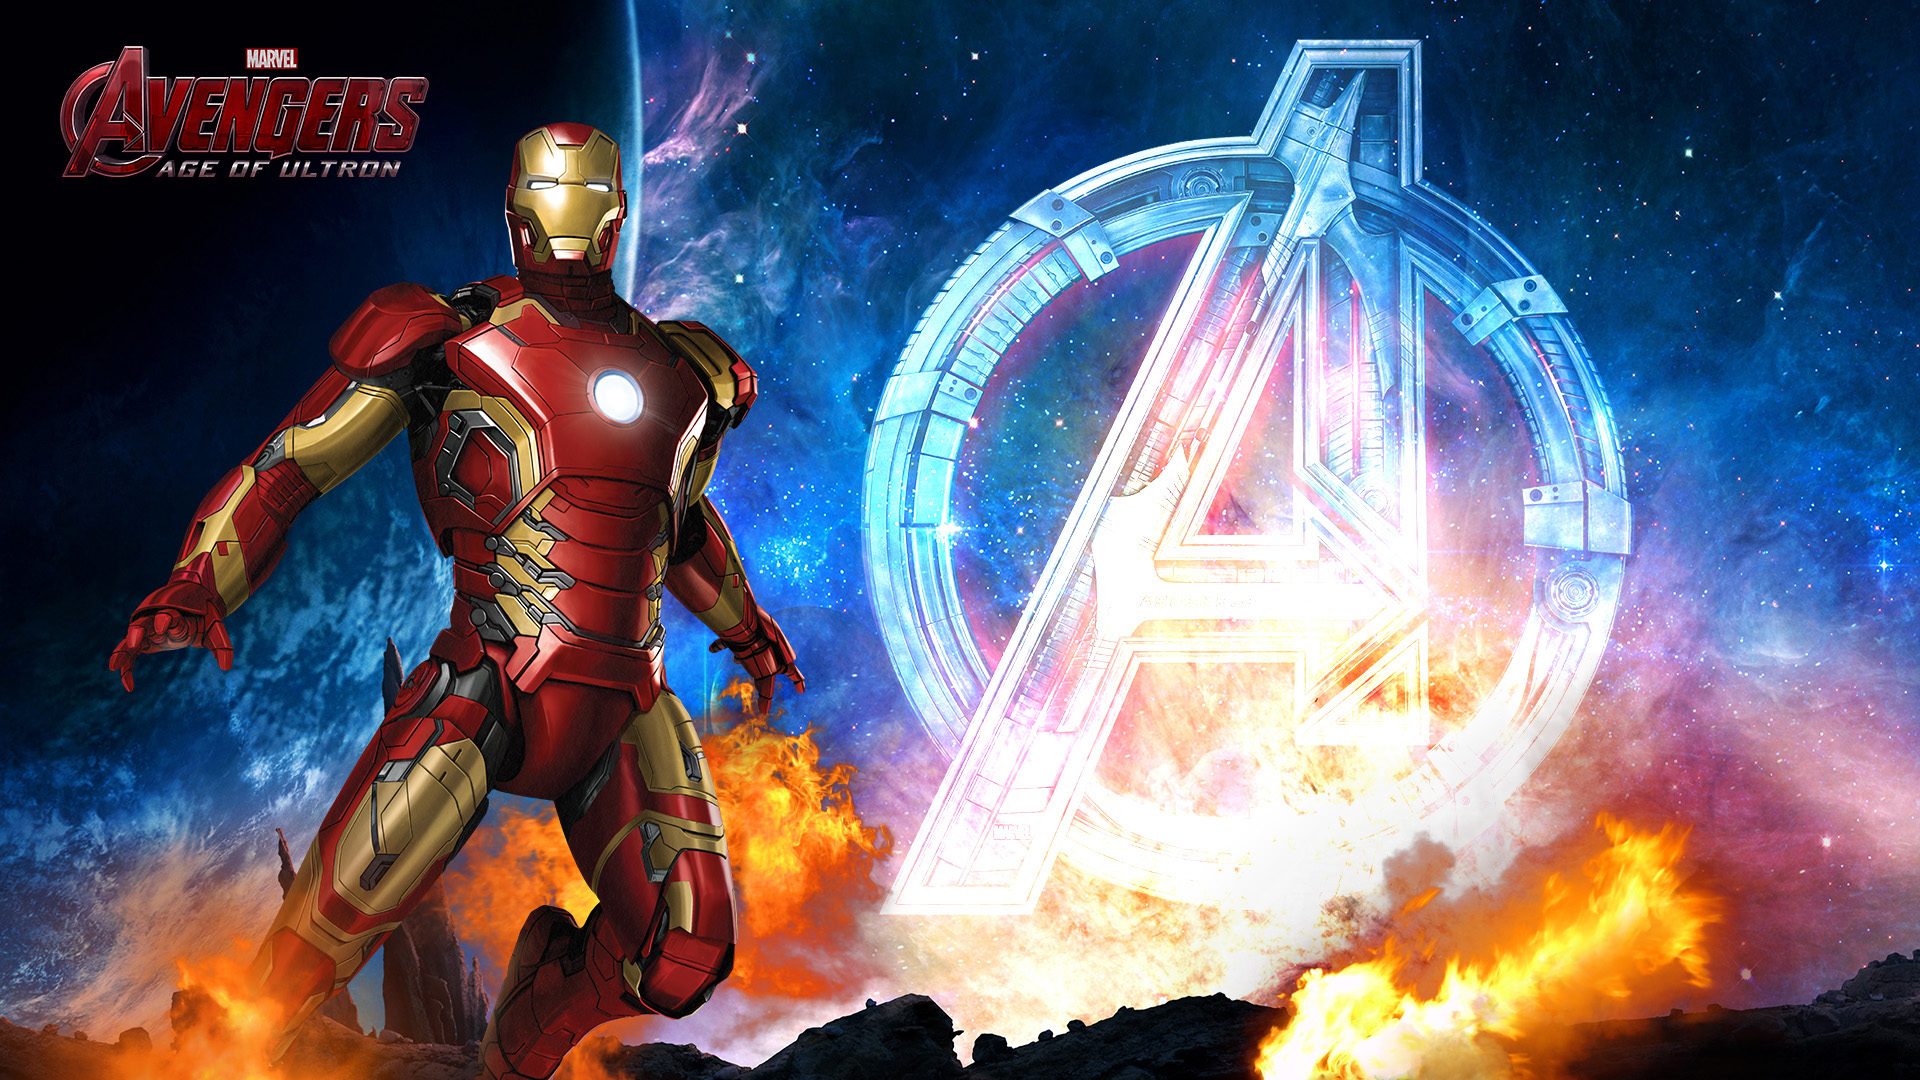
\includegraphics[width=2.5in]{./pictures/6.jpg}
		\label{label_for_cross_ref_2}
	}
	\quad    %用 \quad 来换行
	\subfloat[SubCaption\_3]
	{
		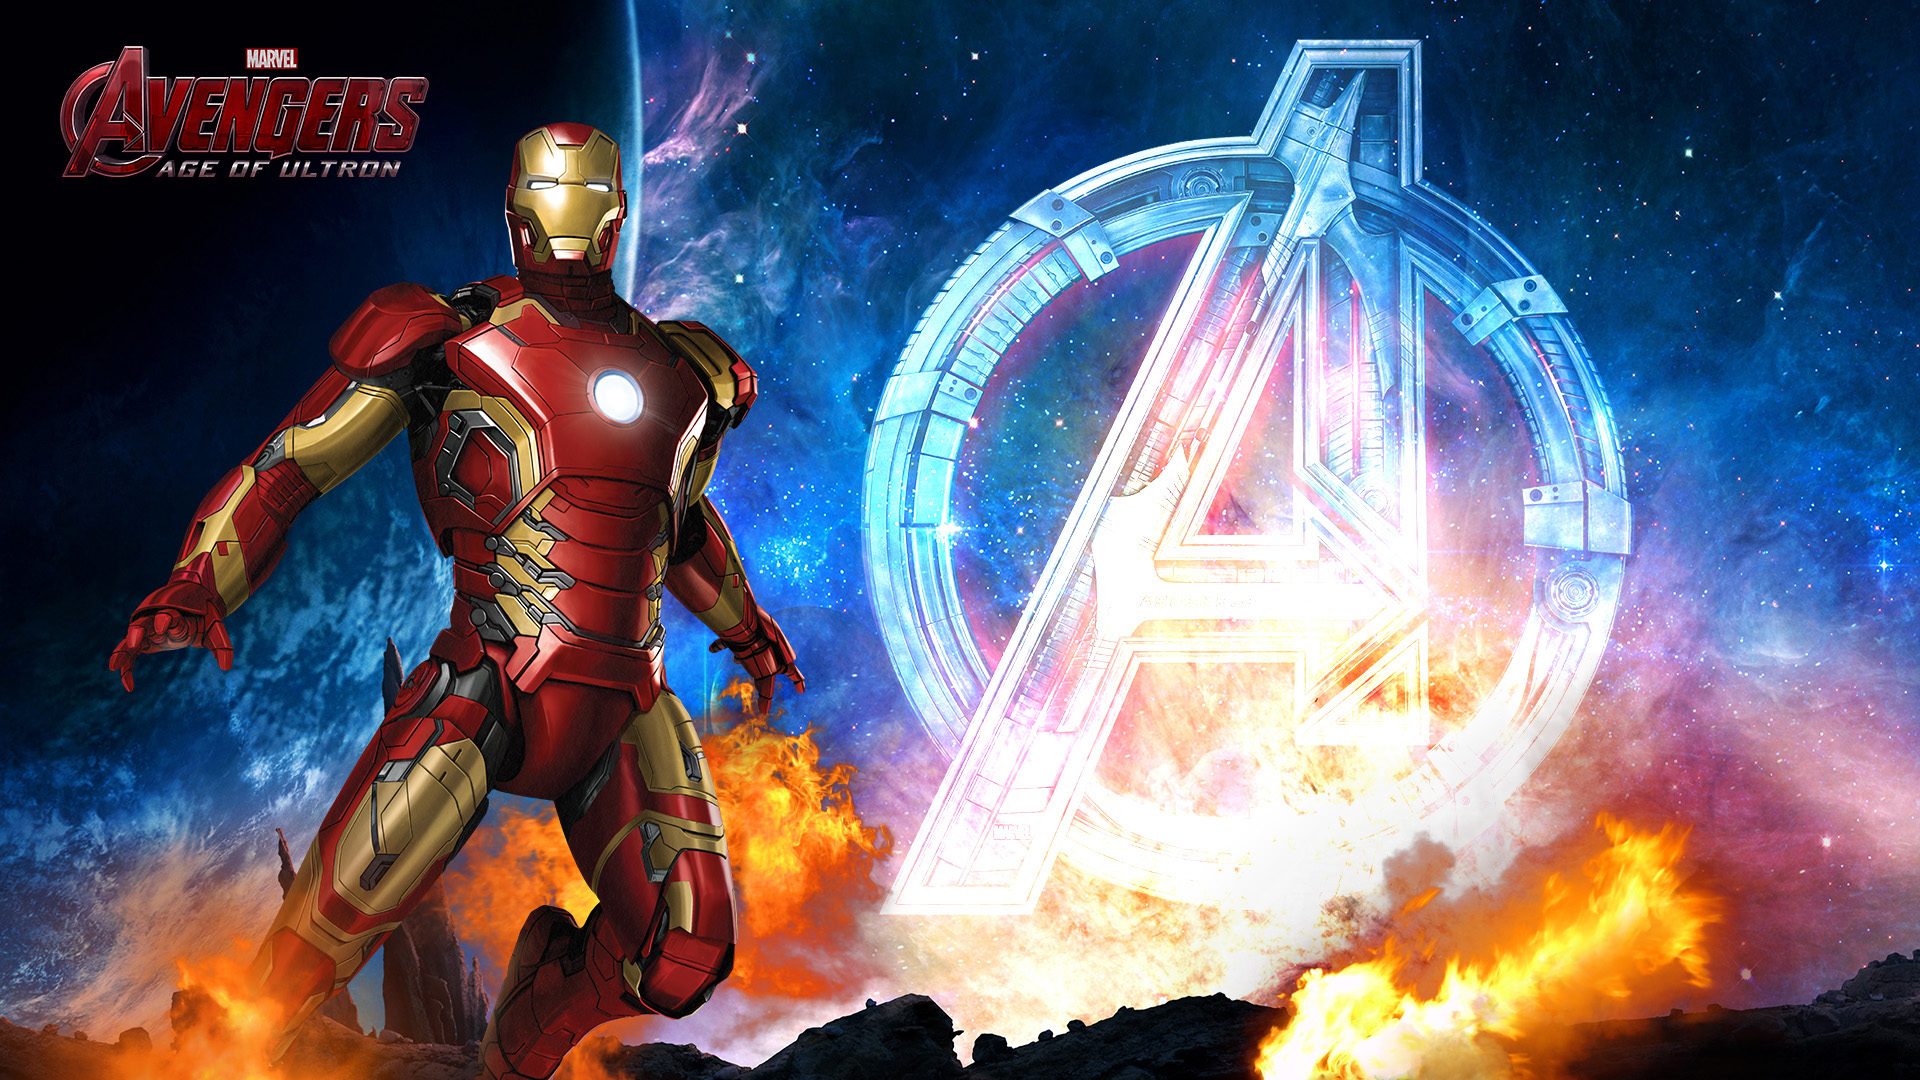
\includegraphics[width=2.5in]{./pictures/6.jpg}
		\label{label_for_cross_ref_3}
	}
	\subfloat[SubCaption\_4]
	{
		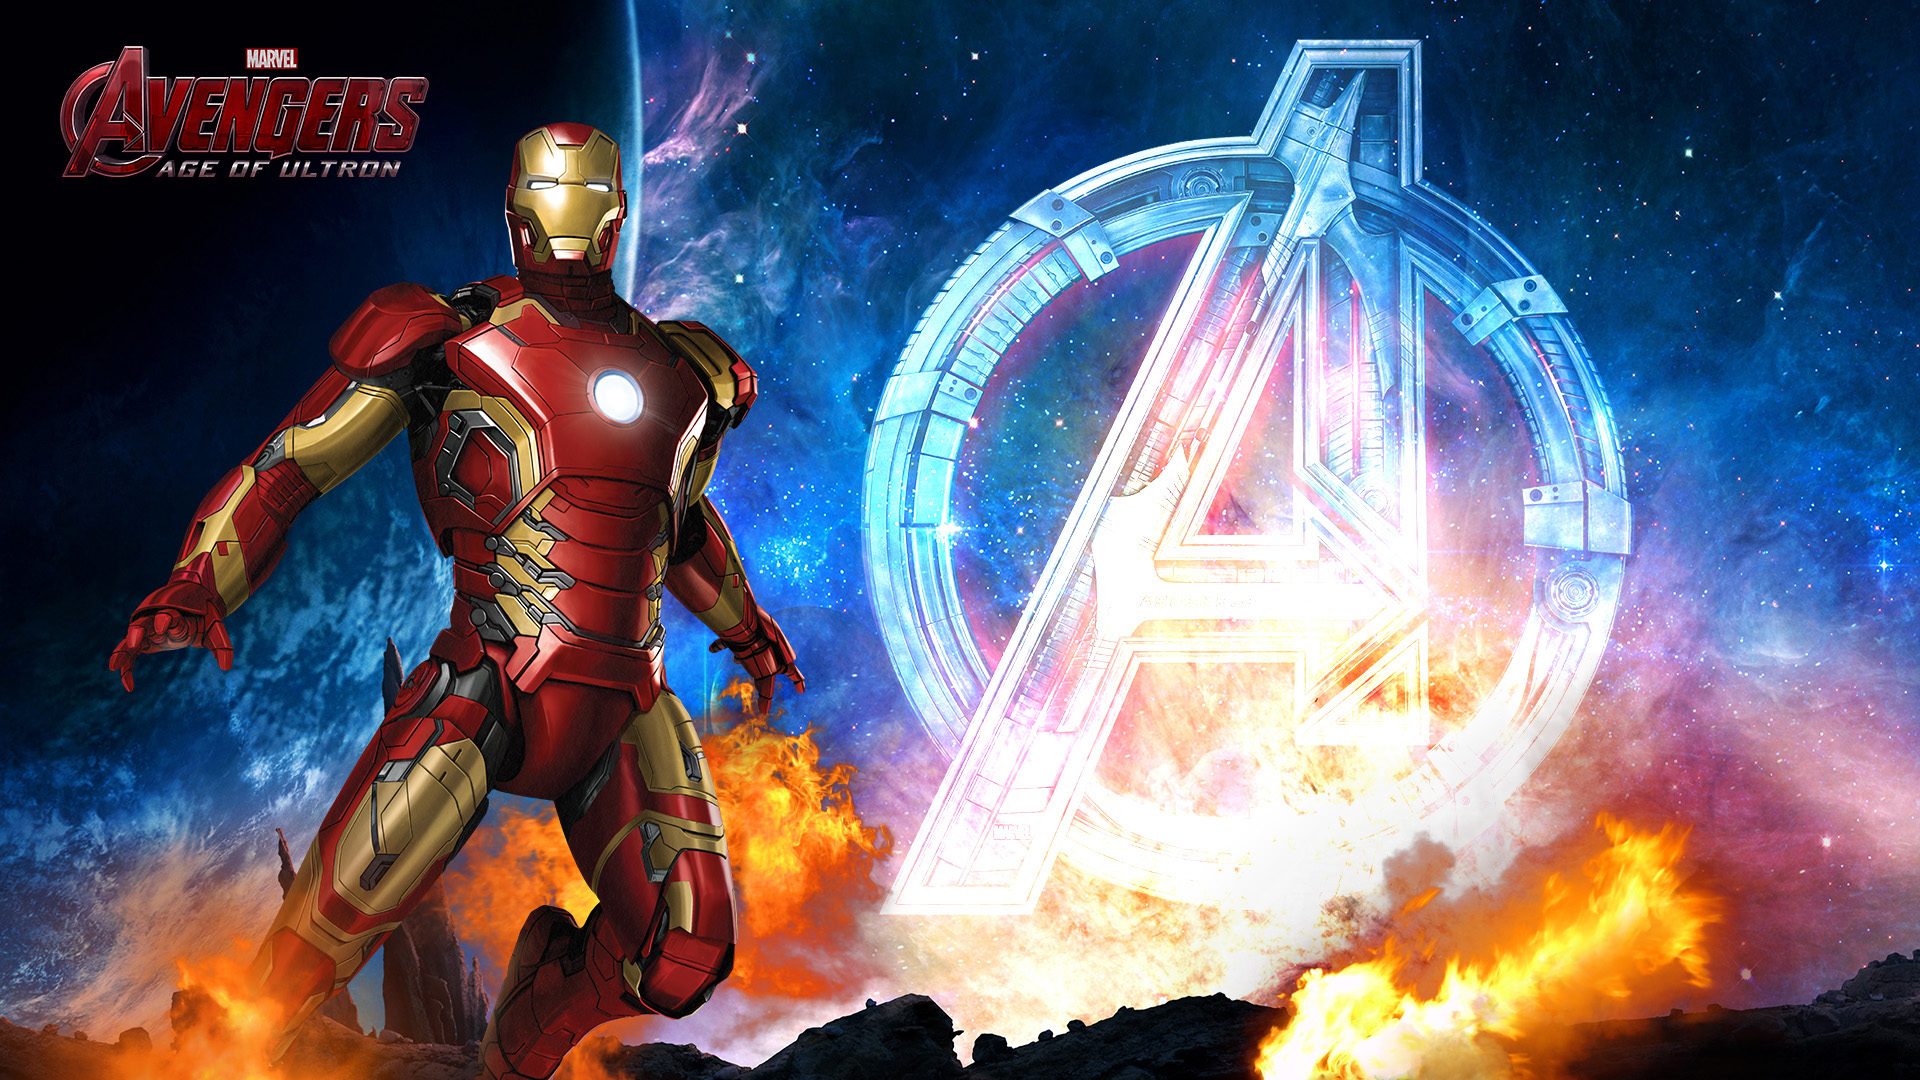
\includegraphics[width=2.5in]{./pictures/6.jpg}
		\label{label_for_cross_ref_4}
	}
	\caption{This is a Demo of $2\times 2$}
	\label{fig.1}
\end{figure}


%% 插入表格
\newpage
\section{插入表格}

可以借助第三方网站:\\
\href{http://www.tablesgenerator.com/latex_tables}{可借助网站工具,点击此字即可}

\begin{table}[!htbp]
	\caption{Nitsche方法的离散误差和误差阶,$f(x,y)=3x-2x^3-2xy^2$。}%{Nitsche's method of discretization errors and error reduction for one-dimensional curve problem.}
	\label{tab:quxianwuchabiaoge_Nitsche}
	\centering
	\footnotesize% fontsize
	\setlength{\tabcolsep}{4pt}% column separation
	\renewcommand{\arraystretch}{1.2}%row space 
	\begin{tabular}{|c|c|c|c|c|c|c|}
		\hline
		网格间距$h$  & $\left \| u^e-u_h \right \|_{L^2(\Gamma)}$ & 阶 & $\left \| u^e-u_h \right \|_{H^1(\Gamma)}$ & 阶 & $\left \| u^e-u_h \right \|_{L^{\infty}(\Gamma)}$ & 阶 \\ \hline
		0.1      & 1.04E-3                                      &    -   & 3.35E-2                                      &    -   & 1.80E-3                                             &   -    \\ \hline
		0.05     & 2.09E-4                                      & 2.31  & 1.51E-2                                      & 1.15  & 4.27E-4                                             & 2.08  \\ \hline
		0.025    & 4.38E-5                                      & 2.26  & 6.96E-3                                      & 1.12  & 1.04E-4                                             & 2.04  \\ \hline
		0.0125   & 1.32E-5                                      & 1.73  & 3.78E-3                                      & 0.88  & 2.81E-5                                             & 1.88  \\ \hline
		0.00625  & 3.08E-6                                      & 2.10  & 1.84E-3                                      & 1.04  & 7.02E-6                                             & 2.00  \\ \hline
		0.003125 & 7.27E-7                                      & 2.08  & 8.99E-4                                      & 1.03  & 1.74E-6                                             & 2.01  \\ \hline
	\end{tabular}
\end{table}


%% else
\newpage
\section{其他}
列表环境:
%%\Alph,\alph,\Roman,\roman,\arabic分别产生A,a,I,i,1
\renewcommand{\labelenumi}{(\roman{enumi})}
\begin{enumerate}
	\item The first item
	\item The second item
	\item The third etc \ldots
\end{enumerate}


\section{第i节}
\subsection{第i.1节}
\noindent % 首行不缩进
《计算机程序设计艺术》第一卷于1968年推出\cite{huang}

\begin{exer}
	好好学习,天天向上。
\end{exer}





\newpage
%% 数学公式等
有编号的公式
\begin{align}\label{eq:1}
\sqrt{a^2 + b^2} &= c^2,\\
\sum_{n=1}^\infty \frac1{n^2}&=\frac{\pi^2}6.\label{eq:2}
\end{align}










\begin{thebibliography}{99}
\bibitem{huang} PDF:黄新刚的\LaTeX Notes:生动有趣
\bibitem{shu} 书籍:刘海洋《\LaTeX 入门》,胡伟《\LaTeX2$\varepsilon$》完全学习手册
\end{thebibliography}

\end{document}